%%%%%%%%%%%%%%%%%%%%%%%%%%%%%%%%%%%%%%%%%%%%%%%%%%%%%%%%%%%%%%%%%%%%%%%%%%%%%%%%
%		      	             __   ____   ___  ____  __ _  ____ 
%                       / _\ (  _ \ / __)(  __)(  ( \(_  _)
%                 		 /    \ )   /( (_ \ ) _) /    /  )(  
%                      \_/\_/(__\_) \___/(____)\_)__) (__) 
%
% Argent Library
% Copyright (c) 2020 Abhishek Chakravarti <abhishek@taranjali.org>
%
% This file is part of the Argent Library. It provides the layout of the manual
% of the Argent Library.
%
% The contents of this file are released under the GPLv3 License. See the
% accompanying LICENSE file or the generated Developer Manual (section I:?) for 
% complete licensing details.
%
% BY CONTINUING TO USE AND/OR DISTRIBUTE THIS FILE, YOU ACKNOWLEDGE THAT YOU
% HAVE UNDERSTOOD THESE LICENSE TERMS AND ACCEPT TO BE LEGALLY BOUND BY THEM.
%%%%%%%%%%%%%%%%%%%%%%%%%%%%%%%%%%%%%%%%%%%%%%%%%%%%%%%%%%%%%%%%%%%%%%%%%%%%%%%%


\documentclass[a4paper, 10pt, twocolumn]{report}

\usepackage[english]{babel}
\usepackage{array}
\usepackage{booktabs}
\usepackage{fontawesome}
\usepackage{graphicx}
\usepackage{imakeidx}
\usepackage{fancyhdr}
\usepackage[backend=biber, bibencoding=utf8, minbibnames=5, maxbibnames=5,
    style=alphabetic, citestyle=authoryear]{biblatex}

\fancyhf{}
\fancyhead[LE]{\leftmark}
\fancyhead[RO]{\nouppercase{\rightmark}}
\fancyfoot[LE,RO]{\thepage}

\addbibresource{argent-manual.bib}
\makeindex[columns=3, title=Index, intoc]

\renewcommand{\familydefault}{\sfdefault}
\pagestyle{fancy}

\begin{document}

\begin{titlepage}
  \centering
  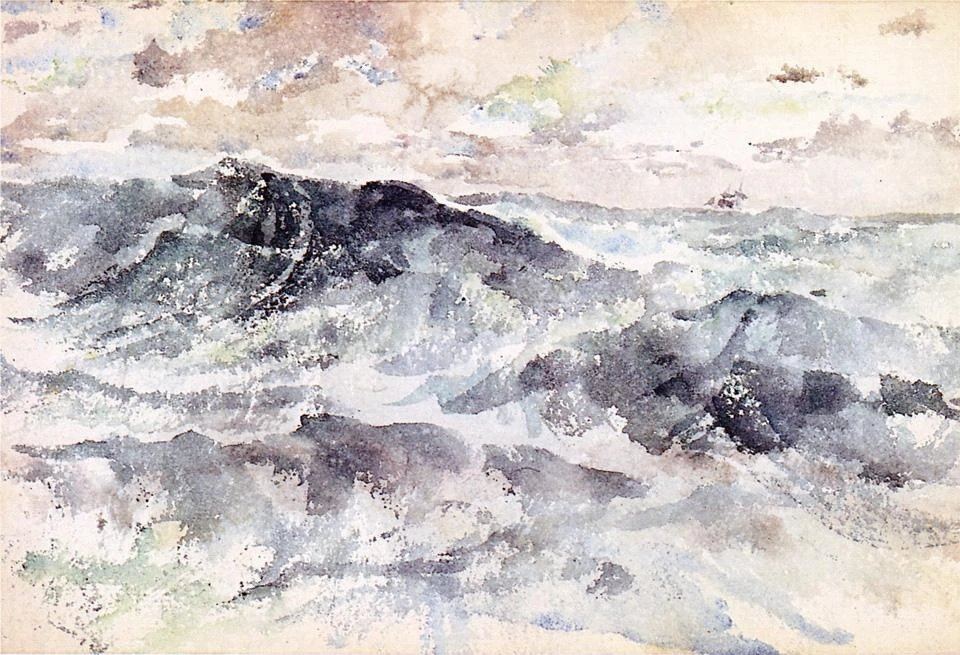
\includegraphics[width=0.95\textwidth]{the-great-sea.jpg}\par \vspace{1em}
  \Huge Argent Library \par \vspace{0.5em} \large v0.1.0 \par \vspace{0.5em} 
      \LARGE Developer Manual \par \vspace{5em} Abhishek Chakravarti \par
      \vspace{0.5em} \small abhishek@taranjali.org \vfill \large May 2020
\end{titlepage}

\tableofcontents
\listoffigures
\listoftables

\part{Overview}
\part{Application Programming Interface}
\part{Implementation}
\part{Test Cases}
\part{Appendix}

\clearpage
\printindex
\end{document}

